\AddToShipoutPicture{\BackgroundPic}

\section*{Principais Características}

Como mencionado anteriormente, o jogo possuirá três etapas que terão dificuldade progressiva. Na etapa de infiltração existirão poucos guardas e será dada maior ênfase aos elementos de navegação do ambiente, especialmente travessias verticais e elementos tradicionais do gênero plataforma. 

	No inicio da segunda etapa o jogador é apresentado à principal mecânica de \emph{stealth} do jogo: ambientes diferentes do atual tem seu interior ocultado do jogador caso sua visão seja obstruida(ver Figura~\ref{visionmode}). Um exemplo seria uma sala com uma porta; caso a porta esteja fechada, a próxima sala não será visível ao jogador, sendo necessário mais cuidado da parte deste ao adentrar o ambiente. 
	
	\begin{figure}[h]
		\center
		\subfigure[refreal][Posicionamento real dos personagens]{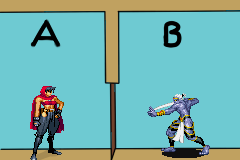
\includegraphics[scale=0.7]{real}}
		\qquad
		\subfigure[refocult][Visão do jogador]{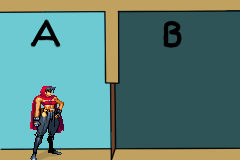
\includegraphics[scale=0.7]{ocult}}
		\caption{Modo de Visão}
		\label{visionmode}
	\end{figure}
	
O jogador terá a possibilidade de olhar através da fechadura da porta para ter uma noção do que o aguarda do outro lado. Nesse modo o jogador terá uma visão em cone da próxima sala, revelando parcialmente o interior da mesma. Baseado nisso ele poderá escolher entre entrar pela porta ou buscar um meio alternativo que ofereça menos riscos.

	\begin{figure}[htb]
		\centering
		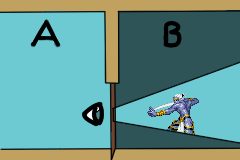
\includegraphics[scale=0.7]{spying}
		\caption{Modo "espião".}
	\end{figure}

Por se tratar de um jogo no qual manter-se oculto é chave, o jogador será capaz de esconder-se atrás de elementos do cenário, como caixas, balcões, árvores ou becos escuros. Também é possível atrair a atenção dos guardas causando perturbações como barulhos, atirando itens do cenário, entre outros. 

	Entretanto, é necessário dar ao jogador maneiras de defender-se e dispor de inimigos ao longo do caminho ou desviar dos mesmos. Para isso ele possuirá equipamentos como um arco, possibilitando ataque a distância, e um gancho, que permite alcançar locais mais altos ou puxar inimigos que estejam próximos um peitoral de janela, por exemplo. O jogador também irá possuir uma opção não letal para dispor de inimigos. 

	A terceira etapa consistirá em navegar o restante do castelo até a sala do trono, onde o jogador irá confrontar o mago, que será o único chefe do jogo. Novamente, por se tratar de um jogo de furtividade, o jogador terá como dispor do inimigo utilizando elementos do cenário, favorecendo paciência e estratégia pela parte do jogador. Após vencer o chefe, o jogo irá terminar e mostrar estatísticas sobre o \emph{playthrough} (tempo, número de vezes que foi encontrado, etc).

